\section{Nuclear Excitation Patterns}

\begin{example}{2}{2-5: Exploring \(\gamma\) Transition Energy Ratios}
\allbold{The ratios \(r_6\) and \(r_8\) are defined for nuclei which approximate an ideal rotor as \[r_6 = \frac{E(6^+_1) - E(4^+_1)}{E(2^+_1)} \quad\quad r_4 = \frac{E(4^+_1) - E(2^+_1)}{E(2^+_1)}\]}

\allbold{a.) Extend this study by defining \(r_8\)}
\[r_8 = \frac{E(8^+_1) - E(6^+_1)}{E(2^+_1)}\]

\allbold{b.) Obtain the rotor limit value for \(r_8\)}

Using \(E(I) \propto I(I+1)\) where \(I\) is the total angular momentum quantum number.
\[r_8 = \frac{8(8+1) - 6(6+1)}{2(2+1)} = 5\]
\allbold{c.) Using \ensdf for even-even rare earth and actinide nuclei around \ce{^{172}Yb} and \ce{^{242}Pu}, make a plot of \(r_8\) vs \(r_2\)}
\end{example}

\begin{example}[breakable]{2}{2-6: Nuclear Recoil Correction for Gamma Transitions}
\allbold{To obtain high precision on ratios of level energies as shown in figure \ref{r6_r4} it may be necessary to perform a correction to the gamma-ray energies observed in experiment as gamma-ray emission is a two-body process where the emitting nucleus recoils. So some small part of the transition energy is taken up by the recoil.}

\allbold{a.) Given that the photon's energy and momentum are related by \(E=pc\), make use of energy and momentum conservation to derive a formula for the nuclear recoil energy as a function of gamma-ray energy, \(E_\gamma\) and atomic mass, \(A\) of the recoiling nucleus.}

By conservation of momentum 
\[\begin{split}
    p_\gamma &= p_{\text{nuc}}\\
    \frac{E_\gamma}{c} &= p_{\text{nuc}}
\end{split}\]
So then the recoil energy of the nucleus will be
\[E_{\text{recoil}} = \frac{p_{\text{nuc}}^2}{2m_{\text{nuc}}} = \frac{E_\gamma^2}{2Ac^2}\]
where \(A\) is in amu. So for the units to work out, use \(c^2 = 931.5 \times 10^6 \,\text{eV/u}\).

\allbold{b.) Estimate the magnitude of the recoil correction for \(A=240\) and \(E_\gamma = 150\) keV.}
\[E_{\text{recoil}} = \frac{(150\times 10^3)^2}{2\times 240 \times 931.5 \times 10^6} = 0.05\,\text{eV}\]

\allbold{c.) Estimate the magnitude of the recoil correction for \(A=12\) and \(E_\gamma = 3213.79\) keV, \(E_\gamma = 4438.94\) keV. Note that these are the energies of \(\gamma\) rays de-exciting the Hoyle state in \ce{^{12}C}. Thus, give your estimate of the excitation energy of the Hoyle state and compare with the value given in \ensdf.}

For \(E_\gamma = 3213.79\) keV:
\[E_{\text{recoil}} = \frac{(3213.79\times 10^3)^2}{2\times 12 \times 931.5 \times 10^6} = 462.00\,\text{eV}\]

For \(E_\gamma = 4438.94\) keV:
\[E_{\text{recoil}} = \frac{(4438.94\times 10^3)^2}{2\times 12 \times 931.5 \times 10^6} = 881.38\,\text{eV}\]

So the total excitation energy of the Hoyle state is
\[3213.79+4438.94+0.462+0.88138 = 7654.07338\,\text{keV}\]
This matches the adopted level from the ENSDF, excerpt below.

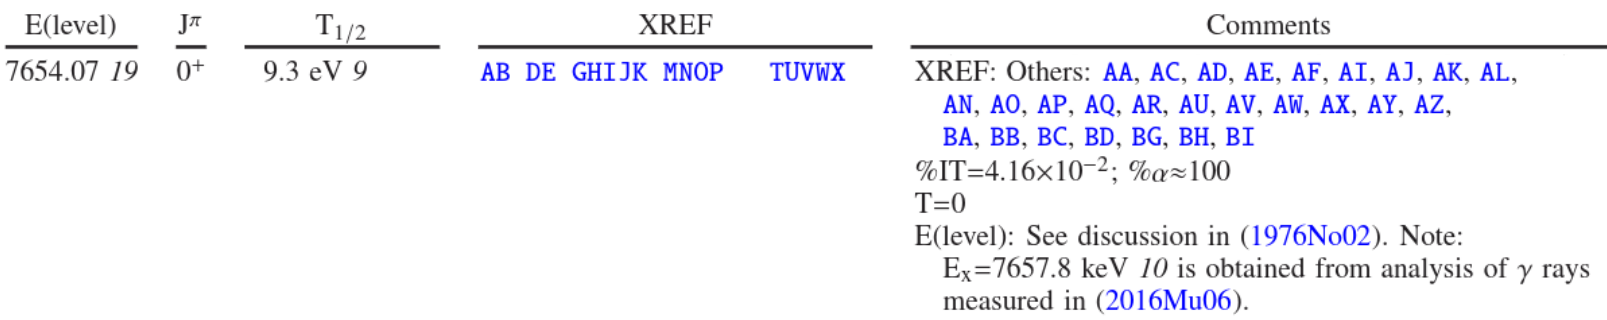
\includegraphics[width=\textwidth]{assets/2.1.2_Hoyle.png}
\end{example}

\begin{example}{3}{2-11: Exploring the Nuclear Structure of \ce{^{152}Sm} with ENSDF Pages}
\allbold{Part 1: Levels}

Looking at adopted levels and gammas. First lot of tables gives the levels. Second lot gives the gammas that connect the levels.

First table gives energy, spin and parity, half life, flags (what reactions it was produced in) and comments. 
Easier to compute separation energies from the AMDC

If spin and parity, \(J^\pi\) is in brackets then its not firmly established. More XREF flags give more confidence. Footnotes contain info on how the data was manipulated but also assignments to different rotational bands. 

f are conversion coefficients, calculated with the bricc tool.

\allbold{Part 2: Matching Data to Levels}

22MeV deuteron scattering experiment. Unpublished so doesn't feature in the ensdf. Magnetic spectrograph used to analyse the scattered deuterons at a fixed angle of 60degrees with a high momentum bite setting. The data has FWHM energy resolution of about 3keV (much lower fidelity than possible by measuring gamma ray transitions with e.g. a high purity germanium detector). Consequently, the 1085 peak is seen as a single peak but is actually two closely spaced levels that aren't resolved 

As to how data is compiled in ENSDF, the energies of excited states are adopted from the highest precision measurements that are available. Usually \(\gamma\) ray transition measurements. For multiple sources, a weighted average of the most precise sources is adopted. To adopt a given excited state energy, a whole network of \(\gamma\) transition measurements is used, both de-exciting and populating a given level. Then, a least-squares fit is taken over the whole network. For \(\gamma\) ray energies with a very high precision (down to eV), then the recoil energy of the nucleus must be added to arrive at the transition energy. 
    
\allbold{Part 3: Matching Data to Transitions Connecting High Spin States}

Here we consider two data sets - Coulomb excitation (coulex) and the nuclear reaction \ce{^{150}Nd(\alpha, 2n\gamma)^{152}Sm}. \(I_\gamma\) is the relative intensity, where 100 is the strongest transition observed. The internal conversion coefficients, \(\alpha\), are calculated using BrIcc, not measured. They are larger for low energy transitions and for high \(Z\) nuclei. Yrast states are the lowest energy states of a given angular momentum, forming the ground state rotational band. 


\end{example}

